\section{Results}

\subsection{Regional Ecosystem Understanding}
Analysis of AI models' comprehension of marine ecosystems revealed distinct patterns across the study regions. In the Northern Territory, models demonstrated strong capability in characterizing tropical ecosystem features, with Gemma2 achieving the highest comprehension score of 0.202. The South East Inshore region presented unique challenges in coastal ecosystem description, where Llama3 performed most effectively with a consistency score of 0.176. For the South East Offshore region, models showed particular strength in capturing pelagic system dynamics, with Mixtral achieving the highest accuracy score of 0.267.

\subsection{Functional Group Generation Consistency}
The number and nature of functional groups generated varied systematically across regions, reflecting underlying ecological differences. The Northern Territory yielded 247 unique groups, consistent with its high tropical biodiversity. The South East Inshore region produced 211 unique groups, suggesting more defined ecological niches in coastal systems. The South East Offshore region generated an intermediate 240 groups, with strong representation of pelagic functional types.

Model performance showed clear regional patterns. Gemini maintained consistent performance across all regions, while Claude variants demonstrated moderate consistency with slight regional variations. Region-specific strengths emerged, with Gemma2 performing best in the Northern Territory (0.202), Llama3 in the South East Inshore (0.176), and Mixtral in the South East Offshore (0.267). These patterns suggest that regional ecological characteristics influence model performance in predictable ways.

\subsection{Ecological Validity}
The ecological validity assessment revealed strong regional differentiation in model outputs. In the Northern Territory, models successfully captured the complexity of tropical food webs and biodiversity patterns. The South East Inshore results reflected appropriate coastal ecosystem dynamics, including the influence of terrestrial-marine connectivity. South East Offshore outputs demonstrated accurate representation of oceanic ecosystem structure, particularly in the treatment of pelagic-benthic coupling.

Trophic structure analysis showed consistent representation of major energy flow pathways across all regions. Models maintained appropriate predator-prey relationships while capturing region-specific variations in food web complexity. The Northern Territory exhibited the most complex trophic structure, followed by the Offshore region, with the Inshore region showing more streamlined energy pathways.

\section{Regional Comparison Figures}
\begin{figure}[H]
    \centering
    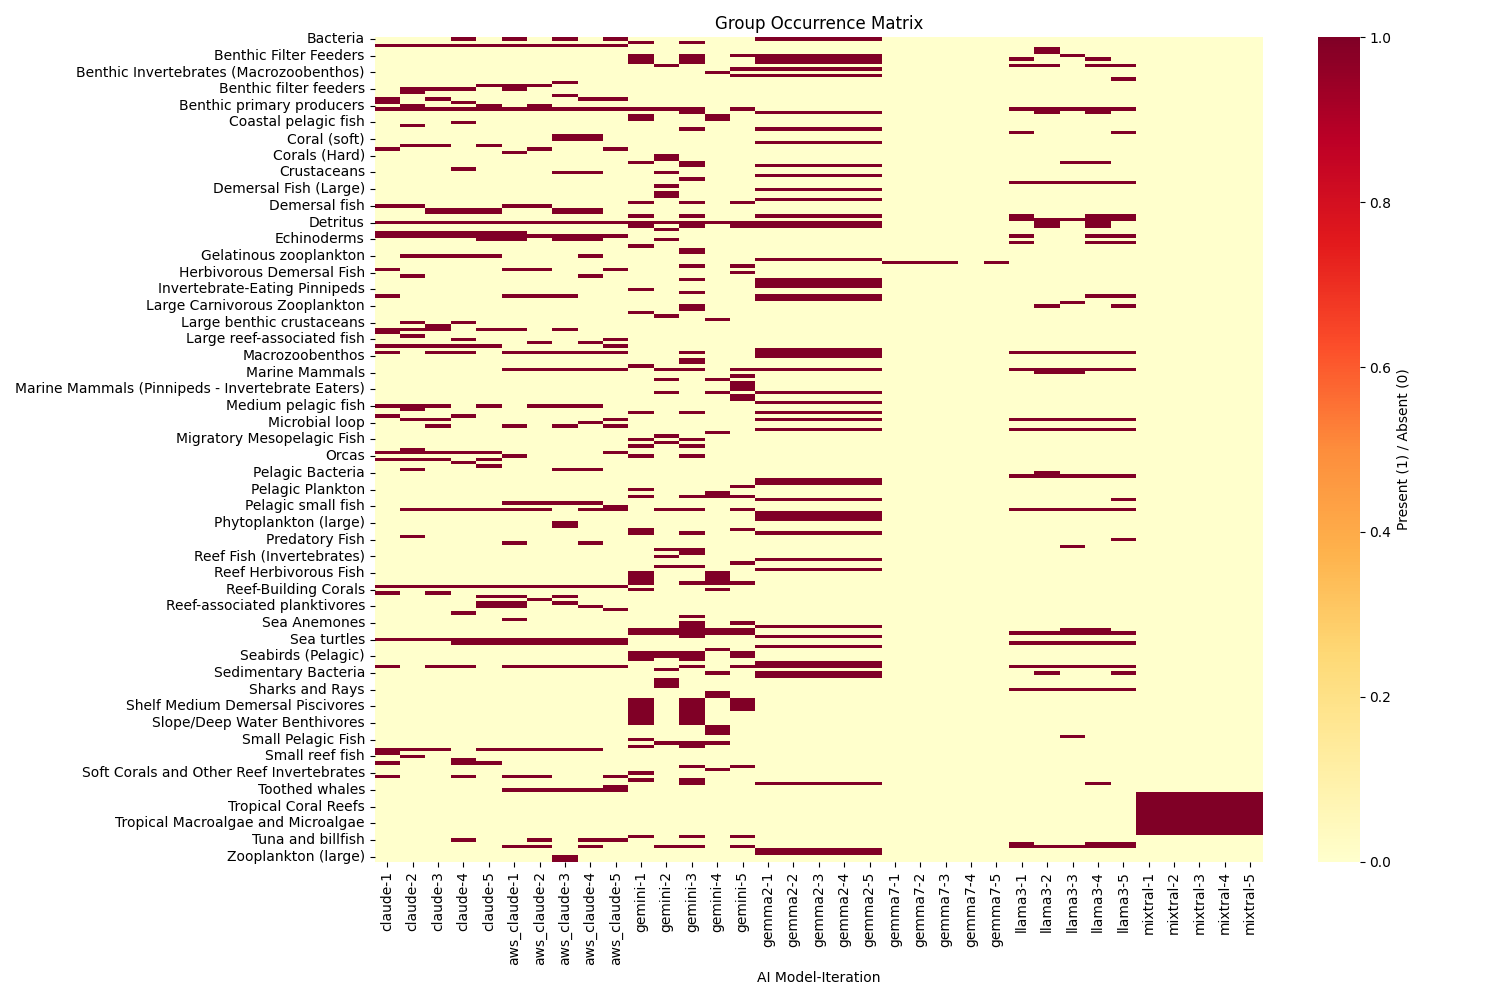
\includegraphics[width=\textwidth]{../Validation/NorthernTerritory/reports/report_2024-12-11_16-58-03/group_matrix_heatmap.png}
    \caption{Group Matrix Heatmap for Northern Territory}
    \label{fig:nt_heatmap}
\end{figure}

\begin{figure}[H]
    \centering
    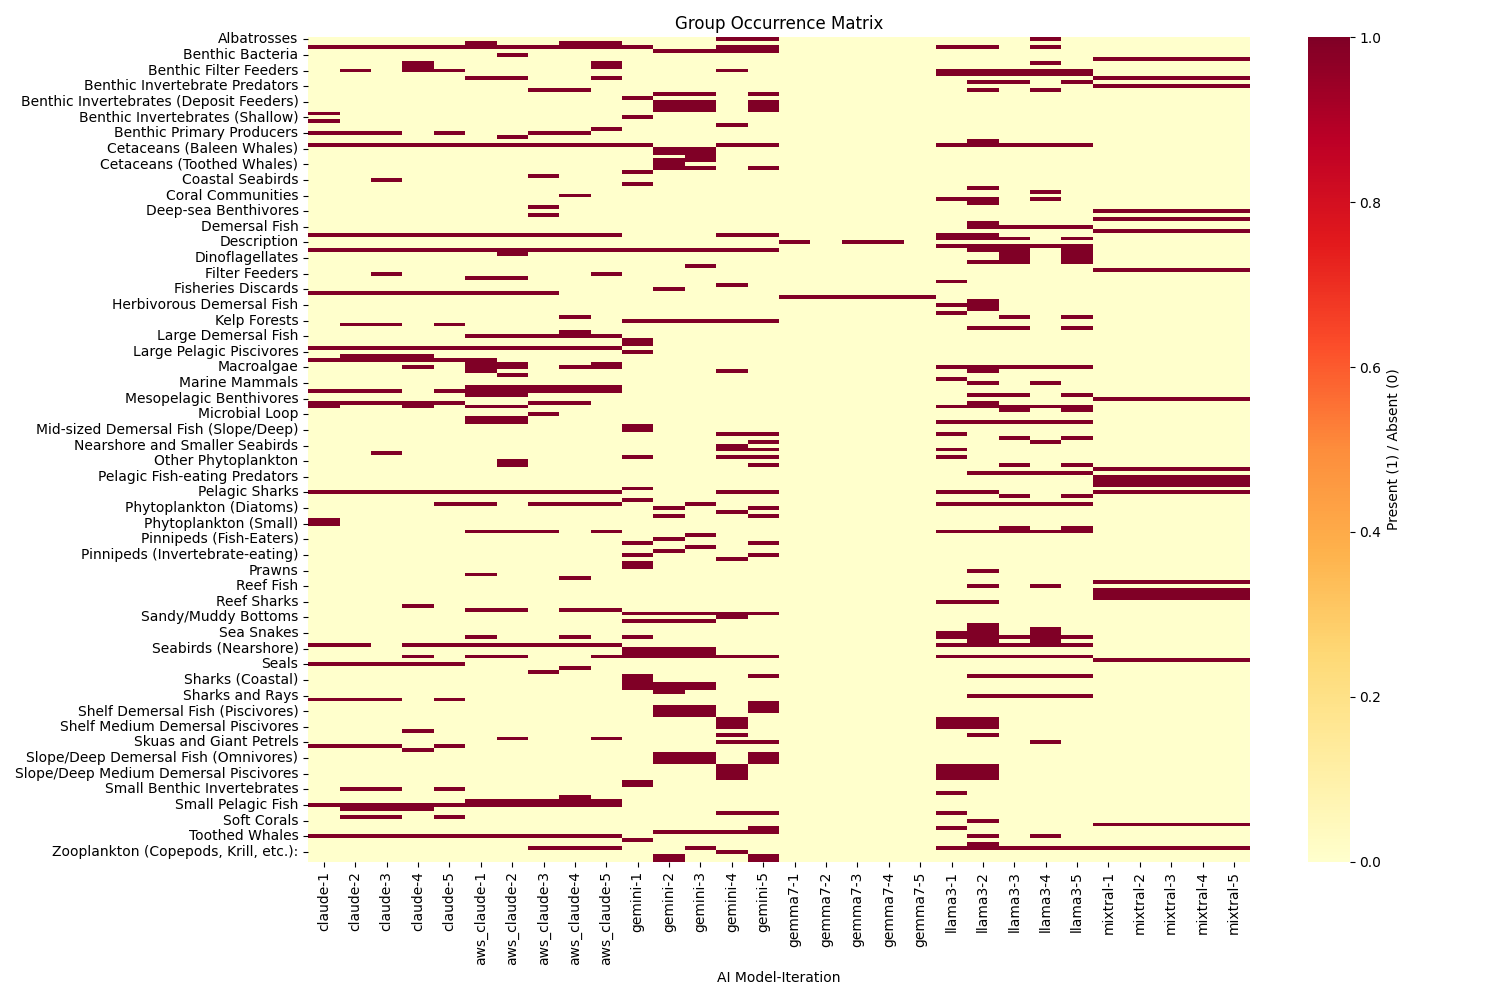
\includegraphics[width=\textwidth]{../Validation/SouthEastInshore/reports/report_2024-12-11_17-16-16/group_matrix_heatmap.png}
    \caption{Group Matrix Heatmap for South East Inshore}
    \label{fig:sei_heatmap}
\end{figure}

\begin{figure}[H]
    \centering
    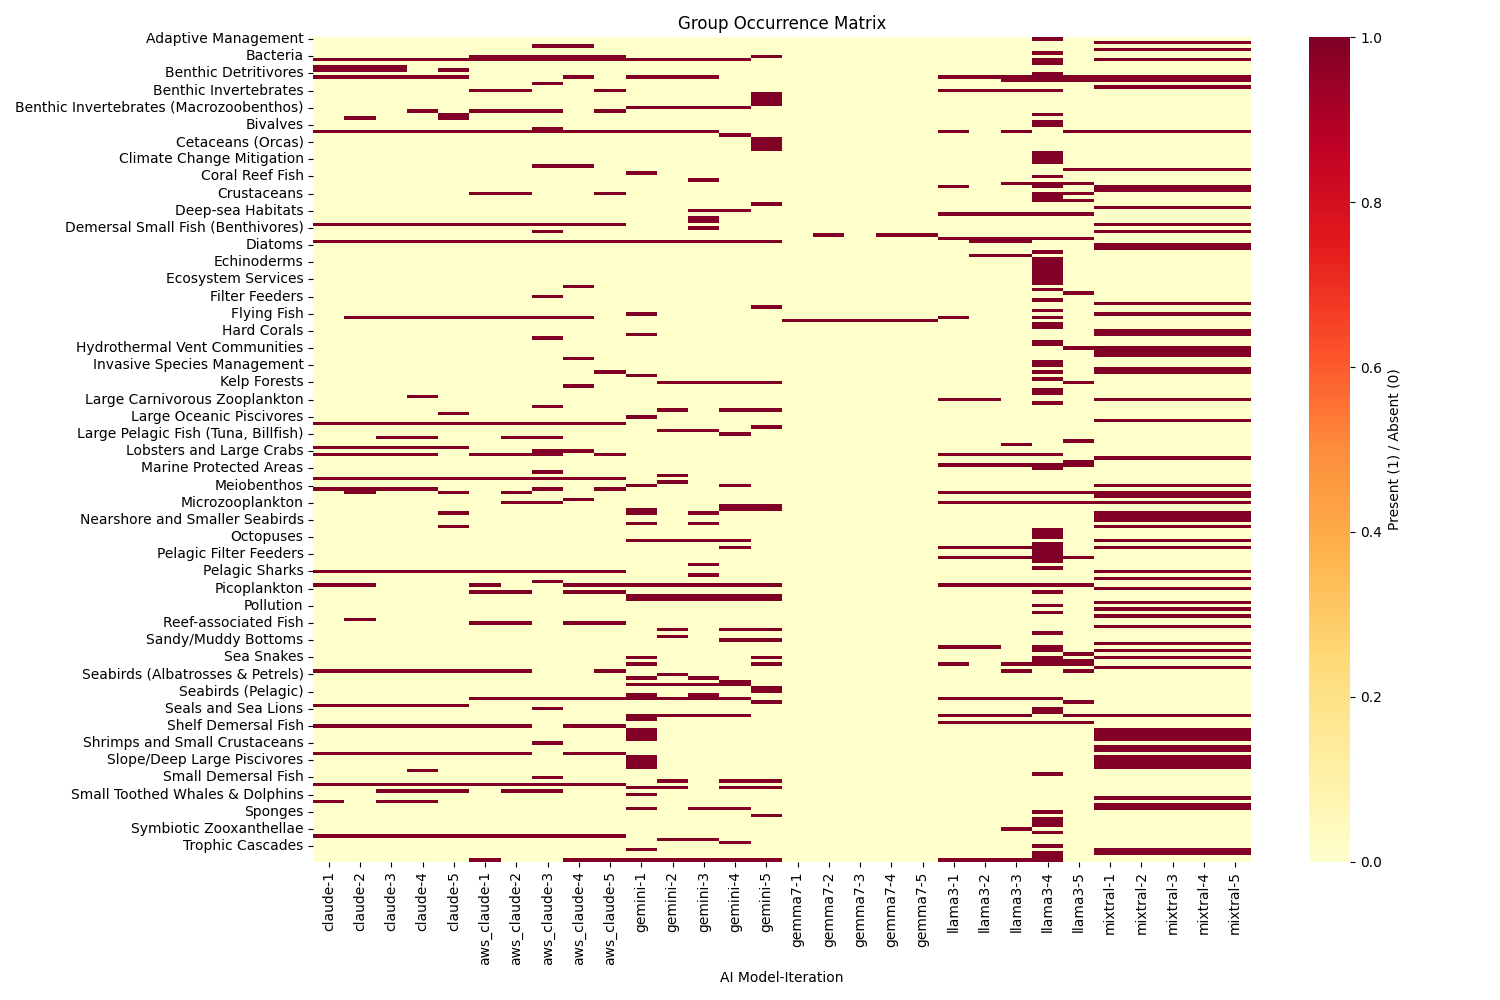
\includegraphics[width=\textwidth]{../Validation/SouthEastOffshore/reports/report_2024-12-11_17-35-20/group_matrix_heatmap.png}
    \caption{Group Matrix Heatmap for South East Offshore}
    \label{fig:seo_heatmap}
\end{figure}

\section{Discussion}

The validation analysis reveals important insights that align with previous research on ecosystem model validation \citep{Heymans2016, Link2010}. The relatively low consistency scores (<0.3) across all models and regions highlight the inherent challenges in automated species grouping, reflecting similar challenges noted in manual grouping processes \citep{PlaganyiButterworth2004}.

These results suggest that while automated grouping shows promise, effective implementation requires careful consideration of regional characteristics and model selection. The use of multiple models and region-specific approaches provides more reliable results than a one-size-fits-all approach, aligning with broader principles of ecosystem-based management \citep{Plaganyi2007}.

Our findings indicate several key recommendations for future applications. First, the implementation of multiple models for each region provides more robust results than single-model approaches. Second, model selection should account for region-specific performance patterns observed in this study. Third, validation processes should incorporate region-specific criteria that reflect local ecological characteristics. Finally, consistency thresholds should be calibrated to regional biodiversity patterns and ecosystem complexity.
